\documentclass[12pt]{article}
\usepackage[margin=1in]{geometry}
\usepackage{graphicx}
\usepackage{caption}
\usepackage{float}
\usepackage{setspace}
\usepackage{booktabs}
\usepackage{siunitx}
\usepackage{amsmath, amssymb}
\usepackage{hyperref}
\hypersetup{colorlinks=true,linkcolor=blue,urlcolor=blue,citecolor=blue}
\sisetup{per-mode=symbol,detect-all=true}
\onehalfspacing
\title{A Computational Analysis of a Set Parameter Beta-Type Stirling Engine\\and Flywheel Design Optimization}
\author{Thomas Ritten \and Sebastian Hondl \and Peyton Lettau}
\date{Group 29 -- ME4051 -- 9/20/25}
\begin{document}
\maketitle
\section*{Abstract}
The effectiveness of an energy conversion system is often defined by its losses: what causes them, how significant they are, and how they can be reduced to improve overall system performance. For Beta-type Stirling engines, we examine work generation in real versus ideal conditions, torque balance across the cycle, crankshaft speed fluctuation, and phase angle sensitivity. We also size a flywheel to meet a target coefficient of fluctuation given material and geometric constraints.

\section{Introduction}
Stirling engines provide a straightforward yet effective method of converting heat into mechanical work. To evaluate performance, we analyze each phase of the cycle versus crank angle \(\theta\), comparing pressure, volume, work, and torque distributions. Beyond the thermodynamic cycle, the flywheel must supply sufficient inertia to maintain near-constant angular velocity without overloading the system.

\section{Given Parameters}
Key parameters used throughout the analysis are summarized below.
\begin{table}[H]
  \centering
  \caption{Initial engine and operating parameters (given).}
  \label{tab:params}
  \begin{tabular}{@{}llll@{}}
    \toprule
    \textbf{Parameter} & \textbf{Symbol} & \textbf{Value} & \textbf{Units} \\
    \midrule
    Power piston crank length & $r_{p}$ & \num{0.025} & \si{\meter} \\
    Power piston connecting rod & $\ell_{p}$ & \num{0.075} & \si{\meter} \\
    Displacer crank length & $r_{d}$ & \num{0.02} & \si{\meter} \\
    Displacer connecting rod & $\ell_{d}$ & \num{0.14} & \si{\meter} \\
    Displacer volume & $V_{d}$ & \num{4.0e-5} & \si{\meter\cubed} \\
    Cylinder bore diameter & $D$ & \num{0.05} & \si{\meter} \\
    Phase shift & $\phi$ & $\pi/2$ & \si{\radian} \\
    Compression ratio & $\mathrm{CR}$ & \num{1.7} & --- \\
    Hot temperature & $T_{h}$ & \num{900} & \si{\kelvin} \\
    Cold temperature & $T_{c}$ & \num{300} & \si{\kelvin} \\
    Gas pressure at BDC & $P_{\mathrm{BDC}}$ & \num{500} & \si{\kilo\pascal} (abs) \\
    Atmospheric pressure & $P_{\mathrm{atm}}$ & \num{101.3} & \si{\kilo\pascal} (abs) \\
    Regenerator dead volume & $V_{\mathrm{reg}}$ & \num{2.0e-5} & \si{\meter\cubed} \\
    Flywheel width & $w$ & \num{0.025} & \si{\meter} \\
    Flywheel rim thickness & $t$ & \num{0.05} & \si{\meter} \\
    Flywheel material density & $\rho$ & \num{8000} & \si{\kilo\gram\per\meter\cubed} \\
    Coefficient of fluctuation & $C_{f}$ & \num{0.003} & --- \\
    Average rotational speed & $\overline{\Omega}$ & \num{650} & \si{rpm} \\
    \bottomrule
  \end{tabular}
\end{table}

% (Section removed to meet 10-page limit; not required by deliverables.)
\section{Methodology}
We begin by discretizing the crank angle as \(\theta \in [0,2\pi)\) with 360 evenly spaced points. With equal bore diameters, the cross-sectional area is \(A = \pi D^{2}/4\).

\subsection{Step 0: Assisting Calculations}
Before analyzing the cycle, we first compute several derived geometric parameters from the given inputs. We calculate the displacer height as \(h_d = V_d/A\) to determine its physical dimensions. Next, we find the power piston positions at bottom and top dead center using the slider-crank equations, which gives us the swept volume \(V_{\text{swept}} = A(x_{\text{TDC}} - x_{\text{BDC}})\). We then determine the total cylinder volume at BDC using the compression ratio: \(V_{\text{total,BDC}} = V_r - V_d + \mathrm{CR} \cdot V_{\text{swept}}/(\mathrm{CR}-1)\). From this, we compute the crank pin to cylinder roof height as:
\begin{equation}
  H_{\text{tot}} = \frac{V_{\text{total,BDC}}}{A} + h_d + h_{\text{pin}} + \ell_p - r_p,
\end{equation}
where the terms account for the cold/hot space height, displacer height, pin offset, and connecting rod geometry. Finally, we set the regenerator temperature \(T_r = (T_h + T_c)/2\). These calculations establish the complete engine geometry needed for the kinematic and thermodynamic analysis that follows.

\subsection{Step 1: Slider--Crank Kinematics}
Then, to begin the analysis, we calculate piston and displacer positions using slider--crank kinematics with rod obliquity. For a crank radius \(r\) and rod length \(\ell\):
\begin{align}
  \beta(\theta) &= \arcsin\!\biggl( \frac{r}{\ell}\,\sin\theta \biggr),\label{eq:beta-def}\\
  x(\theta) &= \ell\,\cos\beta(\theta) - r\,\cos\theta.
\end{align}
We then apply this to get \(x_{p}(\theta)\) for the power piston and \(x_{d}(\theta+\phi)\) for the displacer (phase shifted by \(\phi\)).

\subsection{Step 2: Cold/Hot Volumes}
Next, we compute the cold and hot space volumes from the piston positions. Cold height is the separation between displacer and power piston; hot height is measured from the top space above the displacer:
\begin{align}
  h_{c}(\theta) &= \bigl[x_{d}(\theta+\phi) - x_{p}(\theta)\bigr] - h_{\mathrm{pin}} - \tfrac{1}{2}h_{d},\\
  h_{h}(\theta) &= H_{\mathrm{tot}} - \tfrac{1}{2}h_{d} - x_{d}(\theta+\phi),
\end{align}
which then gives us volumes
\begin{align}
  V_{c}(\theta) &= A\,h_{c}(\theta), & V_{h}(\theta) &= A\,h_{h}(\theta), & V_{r} &= \text{const}.
\end{align}

\subsection{Step 3: Schmidt Analysis and Mass from BDC}
Now we determine the total gas mass and pressure distribution. We start by setting the total gas mass at a known reference point—bottom dead center (BDC, \(\theta=0\))—using the known absolute pressure \(P_{\mathrm{BDC}}\):
\begin{align}
  m &= \frac{P_{\mathrm{BDC}}}{R}\biggl( \frac{V_{c}(0)}{T_{c}} + \frac{V_{r}}{T_{r}} + \frac{V_{h}(0)}{T_{h}} \biggr).
\end{align}
With this fixed mass, we then calculate the instantaneous absolute pressure at any angle using the Schmidt relation:
\begin{align}
  P(\theta) &= \frac{m\,R}{\dfrac{V_{c}(\theta)}{T_{c}} + \dfrac{V_{r}}{T_{r}} + \dfrac{V_{h}(\theta)}{T_{h}} }.
\end{align}
Finally, we evaluate cycle work numerically as
\begin{equation}
  W = \oint P\,\mathrm{d}V \approx \sum_{k} P(\theta_{k})\,\Delta V(\theta_{k}) \quad \text{(trapezoidal rule)}.
\end{equation}

\subsection{Step 4: Torque with Rod Obliquity}
We then convert pressure to torque. The net axial force on the power piston is \(F_{p}(\theta) = \bigl(P(\theta)-P_{\mathrm{atm}}\bigr)\,A\). Using \(\beta\) from Eq.~\eqref{eq:beta-def} and crank radius \(r_{p}\), the torque becomes:
\begin{equation}
  \tau(\theta) = -\,F_{p}(\theta)\,\frac{r_{p}\,\sin\theta}{\cos\beta(\theta)}.
\end{equation}

\subsection{Step 5: Flywheel Sizing}
Next, we size the flywheel to smooth out torque variations. We start by computing the torque deviation about its mean:
\begin{equation}
  T_{\text{dev}}(\theta) = \tau(\theta) - \overline{\tau}, \quad \text{where } \overline{\tau} = \frac{1}{2\pi}\int_0^{2\pi} \tau(\theta)\,\mathrm{d}\theta.
\end{equation}
We then integrate this deviation to get cumulative energy variation. The energy fluctuation \(\Delta E\) is defined as the peak-to-peak of that signal. This gives us the required inertia:
\begin{equation}
  I_{\mathrm{req}} = \frac{\Delta E}{C_{f}\,\omega_{\!\text{avg}}^{2}}.
\end{equation}
We then model the flywheel as a thick ring (like a washer) with width \(w\), thickness \(t\), density \(\rho\), and outer radius \(R\). Most of the mass is concentrated near the outer edge, giving moment of inertia:
\begin{equation}
  I_{\mathrm{rim}}(R) = \tfrac{1}{2}\,M(R)\,\bigl(R^{2}+R_{\mathrm{in}}^{2}\bigr),\quad M(R)=\rho\,\pi w\,\bigl(R^{2}-R_{\mathrm{in}}^{2}\bigr),\quad R_{\mathrm{in}}=R-t.
\end{equation}
To solve \(I_{\mathrm{rim}}(R)=I_{\mathrm{req}}\), we use a fixed-point iteration. We start from a ring-based guess
\(R^{(0)} = \sqrt{I_{\mathrm{req}}/(\pi\,\rho\,w\,t)} + t/2\). At each step, we evaluate
\(I_{\mathrm{act}} = I_{\mathrm{rim}}\bigl(R^{(k)}\bigr)\), form \(\eta = I_{\mathrm{req}}/I_{\mathrm{act}}\), and rescale:
\begin{equation}
  R^{(k+1)} = R^{(k)}\,\eta^{1/3},\qquad R_{\mathrm{in}}=R^{(k+1)}-t.
\end{equation}
We stop when the relative error \(\lvert I_{\mathrm{act}}-I_{\mathrm{req}}\rvert/I_{\mathrm{req}}\) drops below a tolerance.
Why cube root? For a rim-dominant geometry, inertia scales approximately like \(R^{3}\), so scaling \(R\) by \(\eta^{1/3}\) moves directly toward the required inertia with stable, fast convergence.
Finally, we set diameters \(D_{\mathrm{out}}=2R\), \(D_{\mathrm{in}}=2R_{\mathrm{in}}\) and mass \(M(R)\).

\subsection{Step 6: Energy-Based Dynamics}
Now we simulate how the flywheel affects engine speed. We set the load torque equal to mean engine torque for steady-state operation. The net torque then drives angular acceleration \(\alpha = T_{\text{net}}/I\). Using the work--energy theorem over angle increments with cumulative work \(W_{\text{net}}(\theta)\), we update speed via:
\begin{equation}
  \Omega^{2}(\theta) = \Omega_{\!\text{avg}}^{2} + \frac{2\,W_{\text{net}}(\theta)}{I},\qquad \Omega(\theta) = \sqrt{\Omega^{2}(\theta)}.
\end{equation}
We then normalize \(\Omega\) to recover the target average. This normalization is necessary because the energy-based calculation can drift slightly from the desired mean speed due to numerical integration, so we rescale the entire speed profile to maintain the correct average while preserving the fluctuation pattern.

\subsection{Step 7: Phase Optimization}
Finally, we optimize the phase shift to maximize power output. We perform a three-stage search over \(\phi\): first, a coarse scan from \(30^{\circ}\) to \(150^{\circ}\) in \(2^{\circ}\) steps to find a good neighborhood. Then, we zoom in with a medium scan within \(\pm6^{\circ}\) of the coarse best at \(0.1^{\circ}\) resolution. Finally, we pinpoint the optimum with a fine scan within \(\pm0.5^{\circ}\) at \(0.01^{\circ}\) resolution. At each phase, we compute mean torque integrated over \(\theta\), calculate power as \(\bar{\tau}\,\omega_{\!\text{avg}}\), and select the \(\phi\) that maximizes power.

\section{Results and Discussion}
The computational analysis yields comprehensive results across all aspects of the Stirling engine performance, from kinematic behavior to thermodynamic efficiency and dynamic response. The results are presented following the systematic analysis methodology, beginning with piston kinematics and progressing through thermodynamic analysis, dynamic behavior, and optimization.

\subsection{Piston Kinematics and Volume Analysis}
Kinematics establish the volume envelopes that drive the thermodynamics. The power piston stroke is 50.00 mm and the displacer stroke is 40.00 mm (power piston max position 100.00 mm; displacer 160.00 mm). The total volume spans 140.25–238.42 cm³, giving the specified compression ratio of 1.70. Hot and cold volumes vary between 32.26–110.80 cm³ and 35.61–163.18 cm³, respectively, with a constant 20.00 cm³ regenerator volume. These values set the pressure swing and, ultimately, the cycle work.

\subsection{Thermodynamic Analysis and Pressure-Volume Behavior}
The Schmidt analysis reveals pressure behavior throughout the cycle, with pressure ranging from 474.63 to 1178.83 kPa, a mean pressure of 730.39 kPa, and a pressure ratio of 2.48. This pressure variation is significantly lower than the ideal Stirling cycle due to the presence of dead volumes and the simplified Schmidt assumptions.

Figure~\ref{fig:pv_diagram} compares the actual engine cycle with the ideal Stirling cycle, providing insight into the thermodynamic performance.

\begin{figure}[htbp]
  \centering
  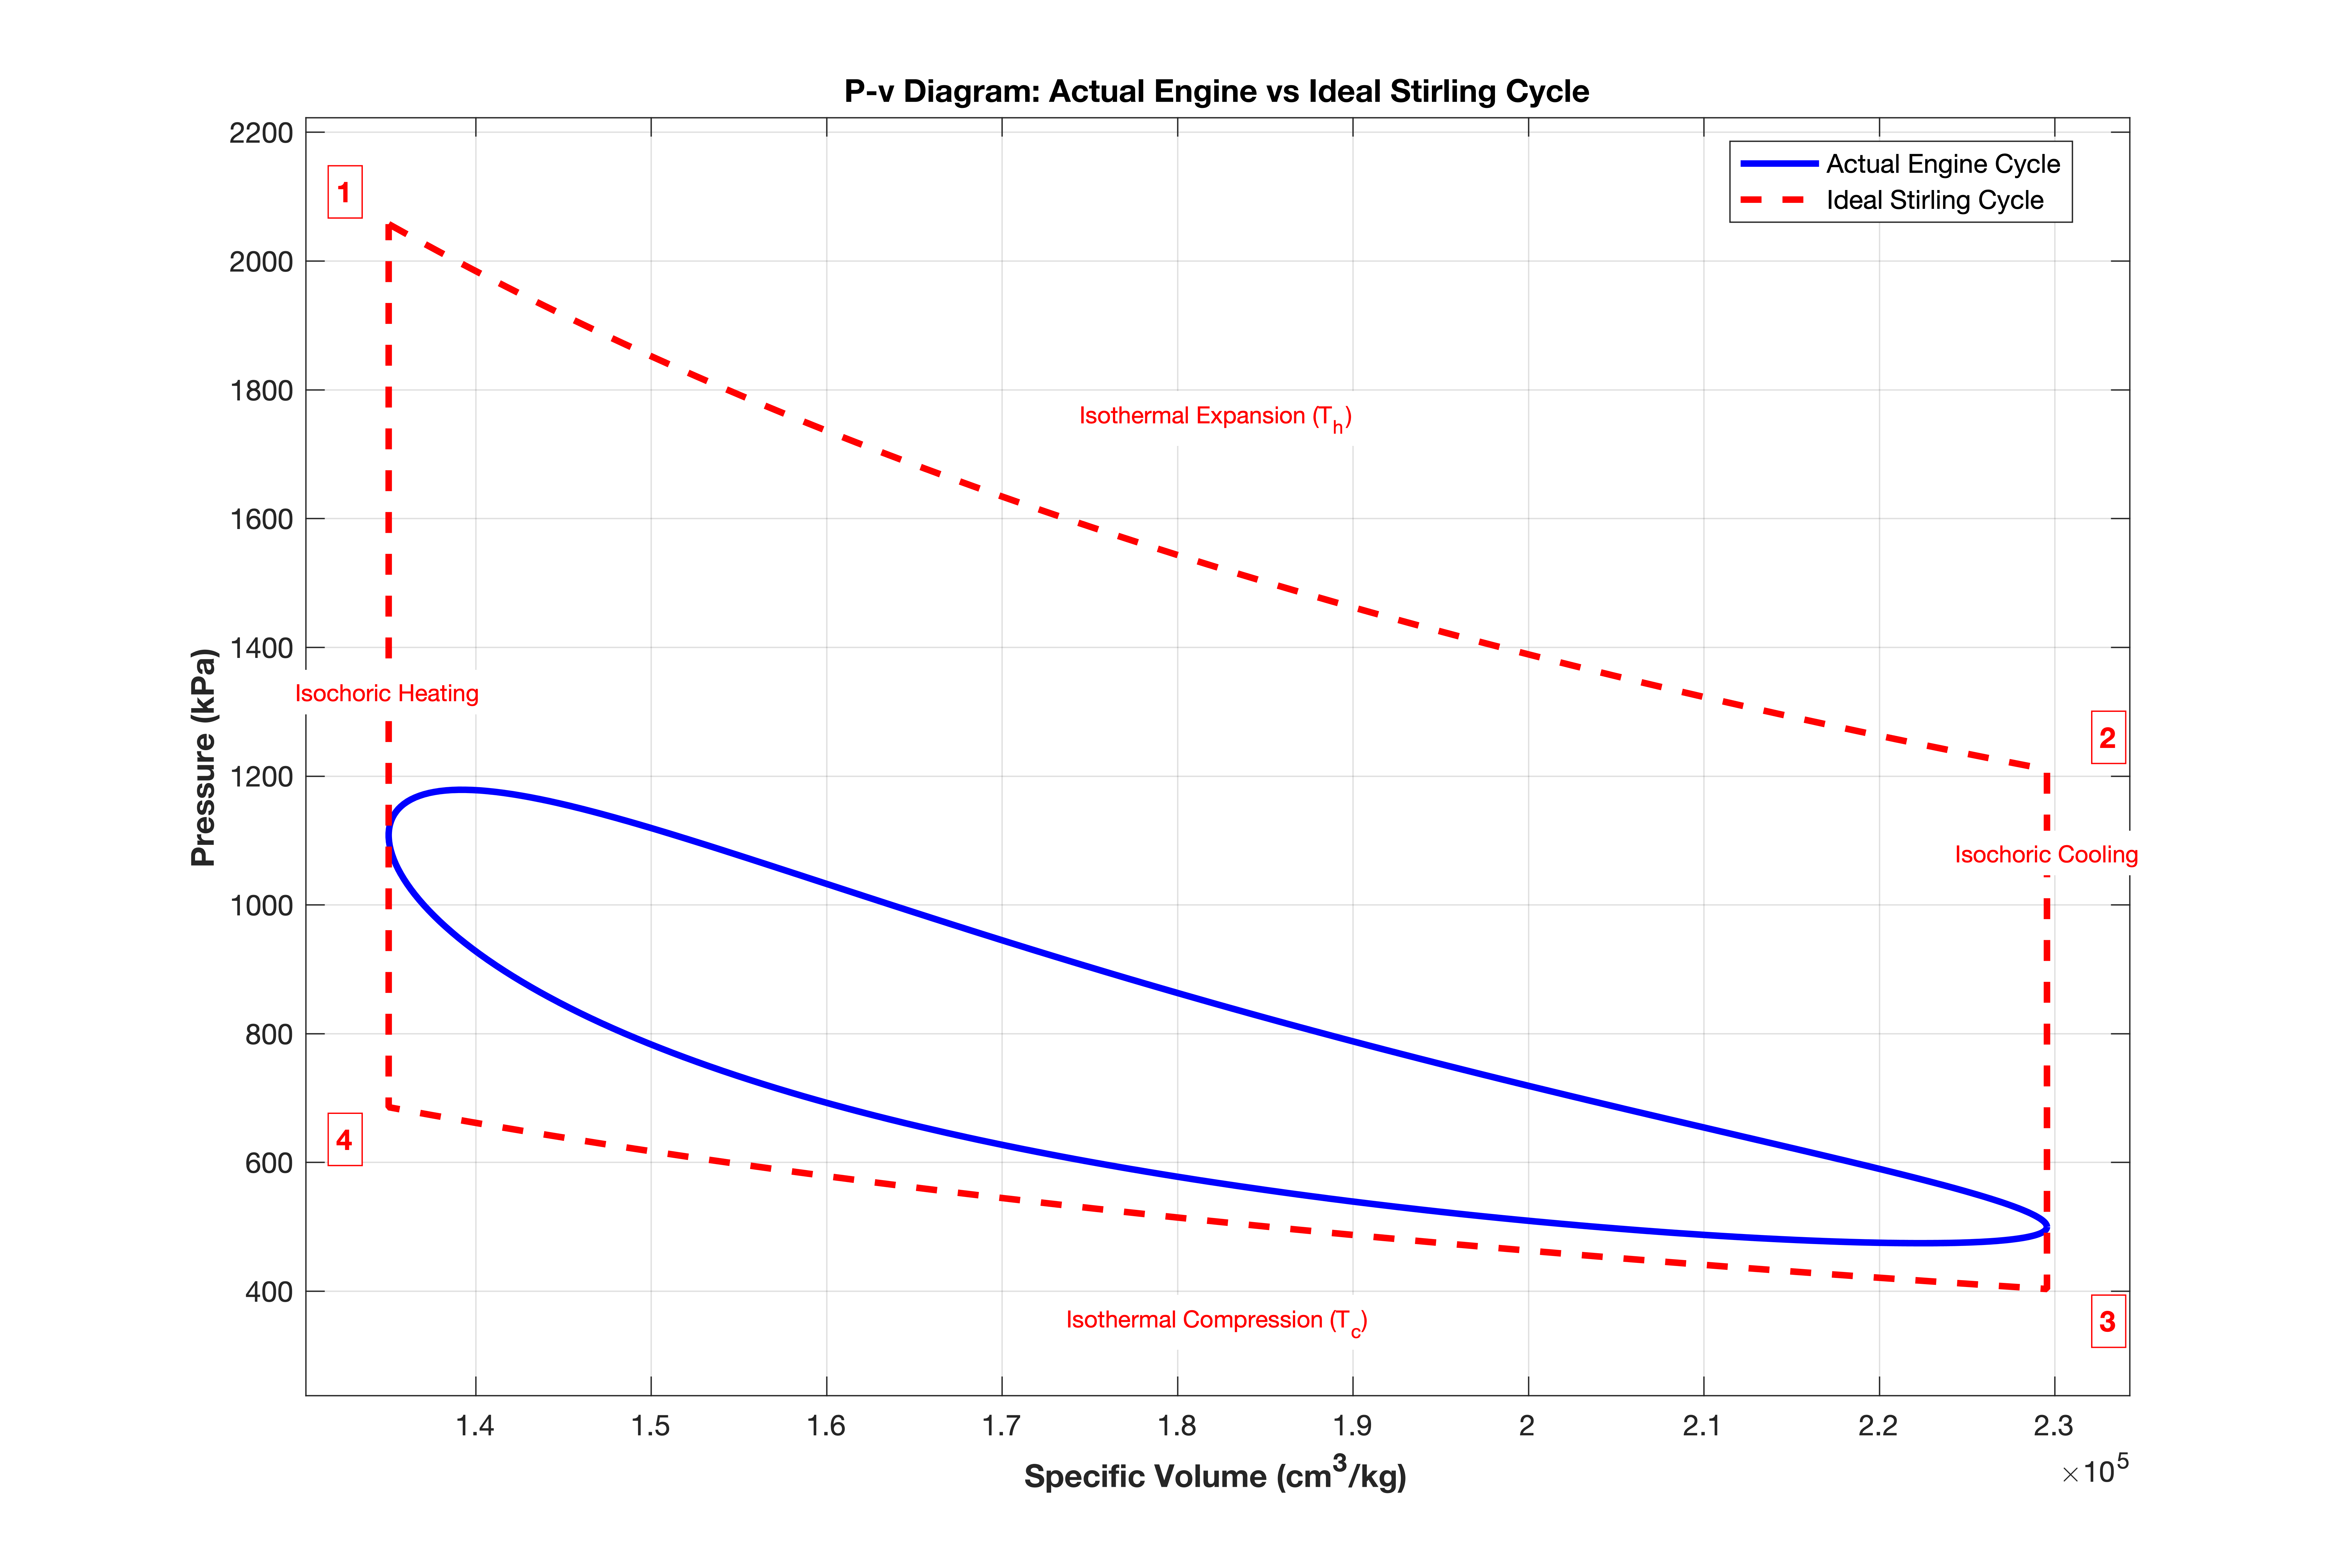
\includegraphics[width=0.8\linewidth]{../pv_diagram.png}
  \caption{P-v diagram comparing the actual engine cycle with the ideal Stirling cycle.}
  \label{fig:pv_diagram}
\vspace{-6pt}\end{figure}

The ideal Stirling cycle produces 94.9 J of work per cycle, while the actual Schmidt analysis yields only 23.0 J, resulting in a cycle efficiency of 24.2\%. This substantial difference highlights the impact of dead volumes, non-ideal heat transfer, and the simplified assumptions inherent in Schmidt analysis.

\subsection{Torque Analysis and Power Production}
The torque analysis, shown in Figure~\ref{fig:torque_angle}, reveals the instantaneous power production capability of the engine.

\begin{figure}[htbp]
  \centering
  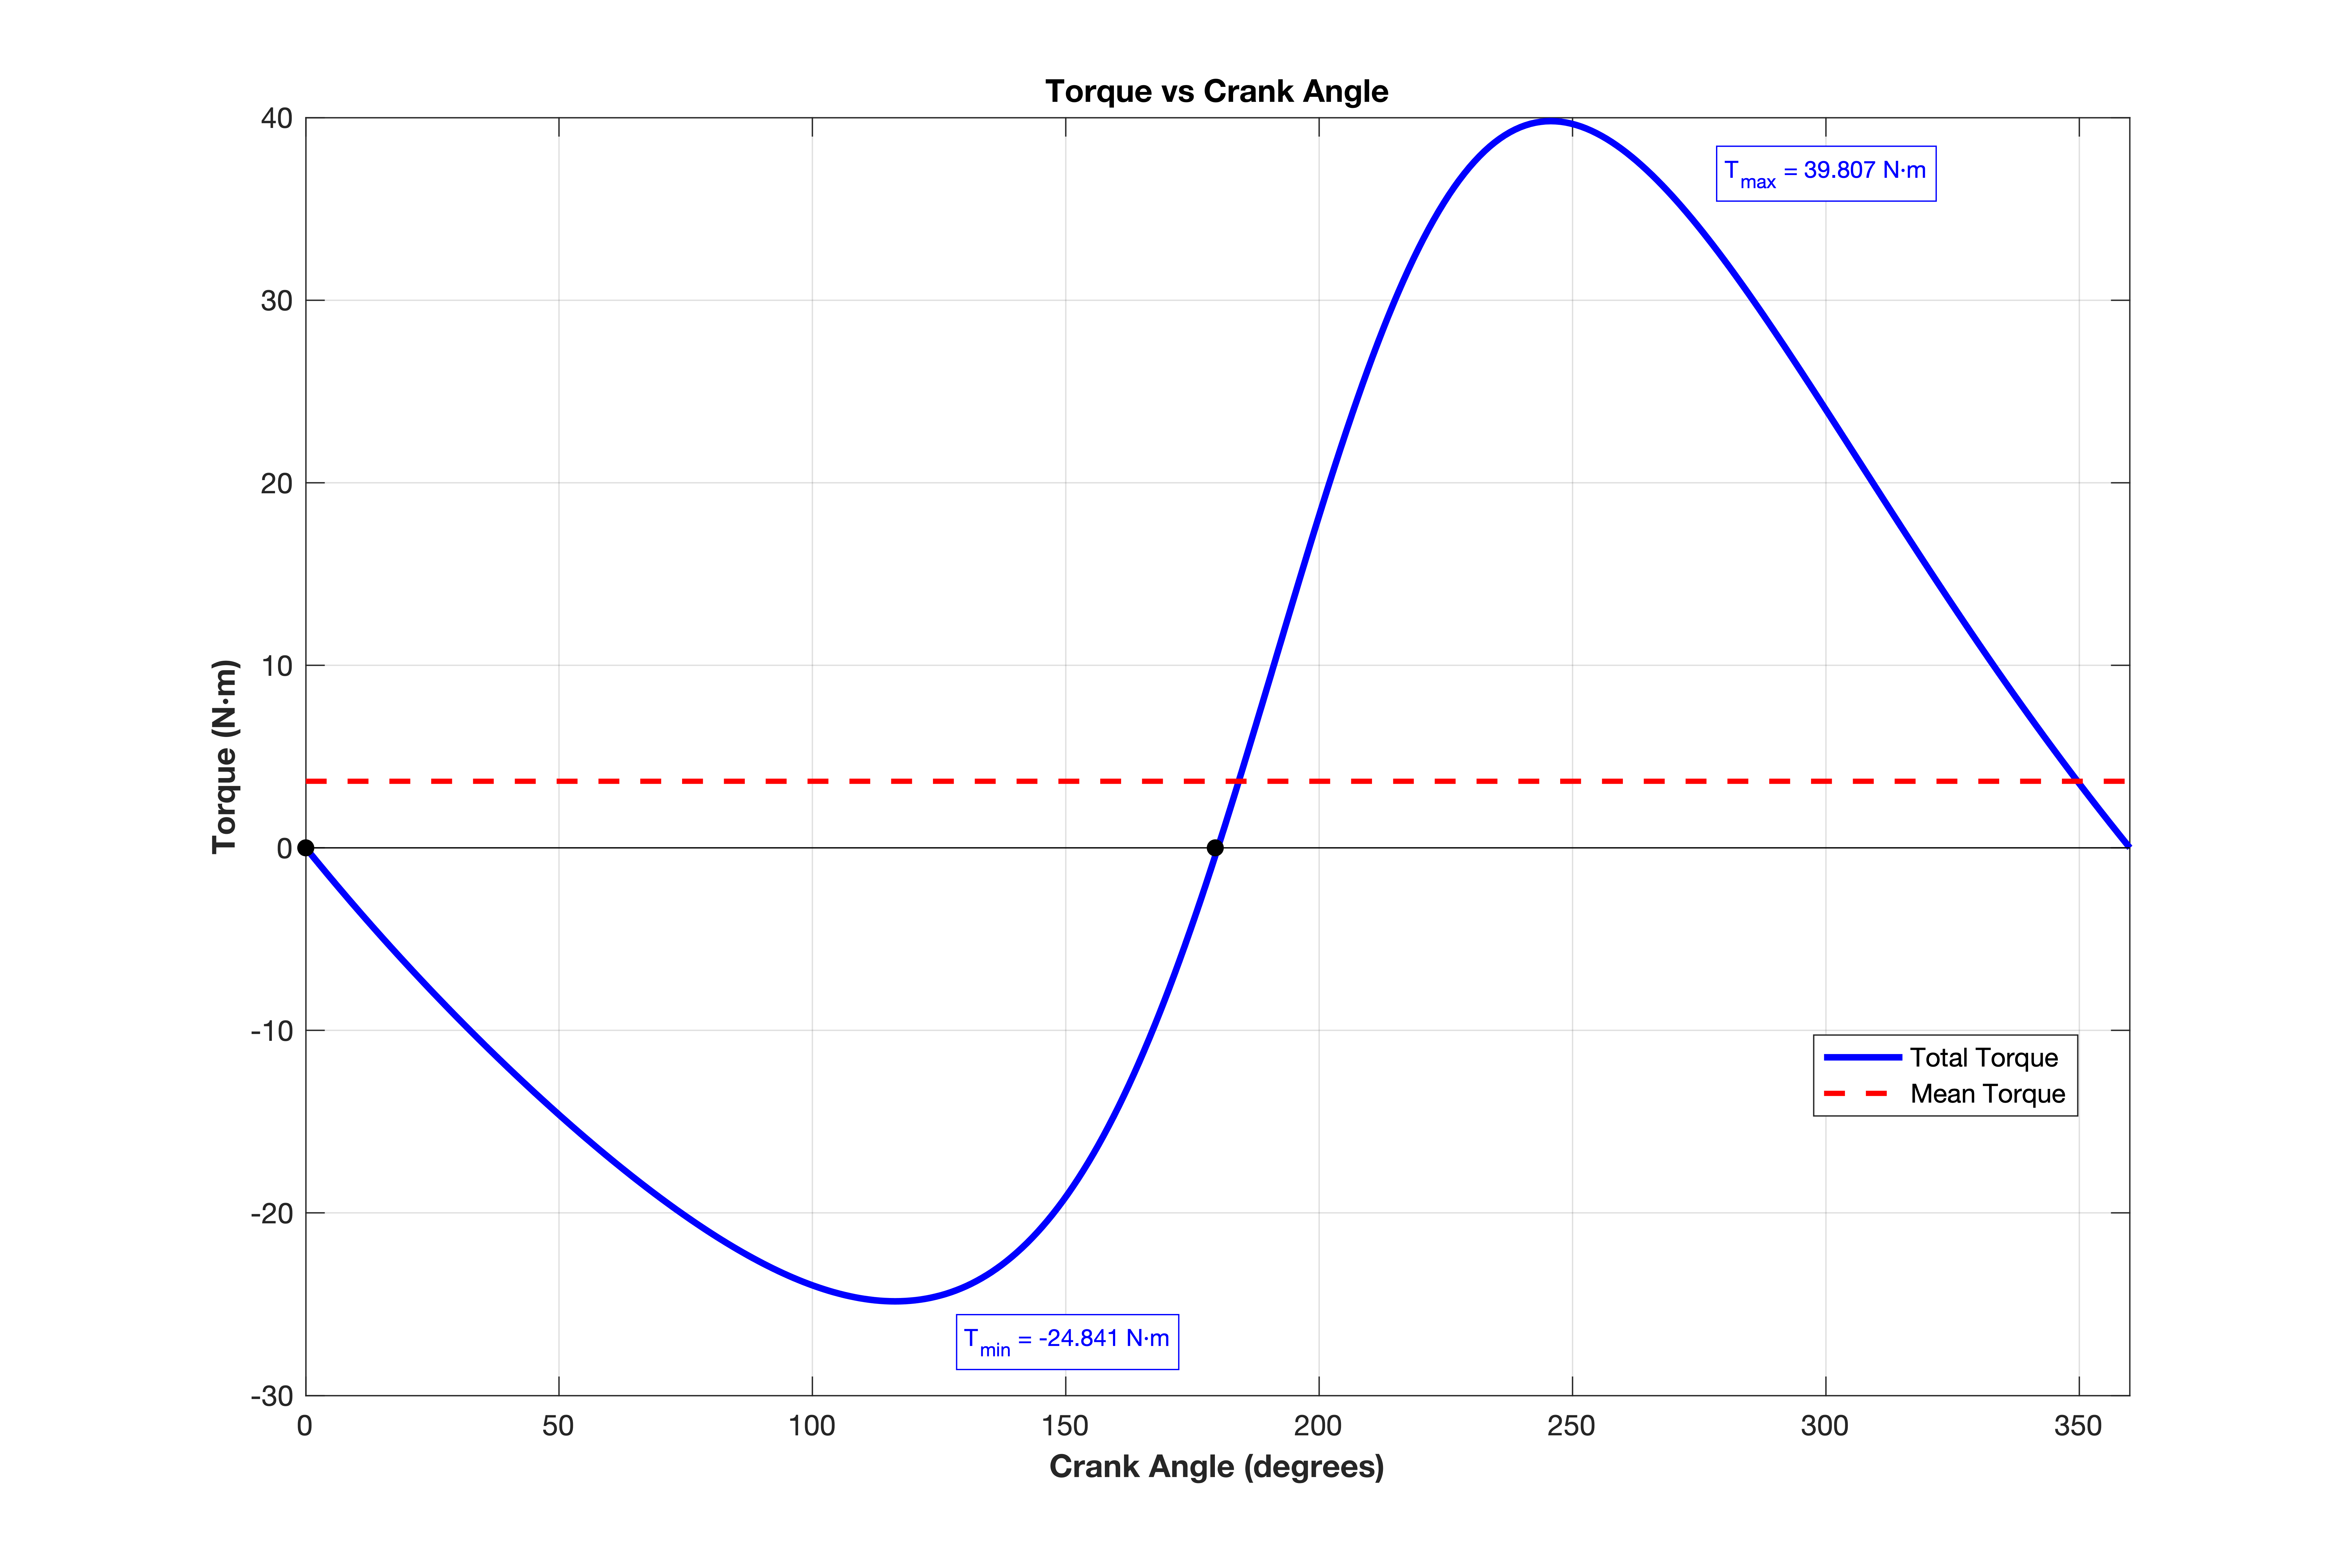
\includegraphics[width=0.8\linewidth]{../torque_vs_angle.png}
  \caption{Torque vs. crank angle showing the instantaneous torque production throughout the cycle.}
  \label{fig:torque_angle}
\vspace{-6pt}\end{figure}

The total torque ranges from -24.841 to 39.807 N·m, with a positive mean torque of 3.648 N·m, confirming the engine's ability to produce net work output. The torque variation reflects the pressure-volume work interaction, with positive torque during expansion phases and negative torque during compression phases.

\subsection{Dynamic Behavior and Flywheel Performance}
The angular velocity analysis demonstrates the effectiveness of the flywheel design in maintaining consistent rotational speed, as shown in Figure~\ref{fig:angular_velocity}.

\begin{figure}[htbp]
  \centering
  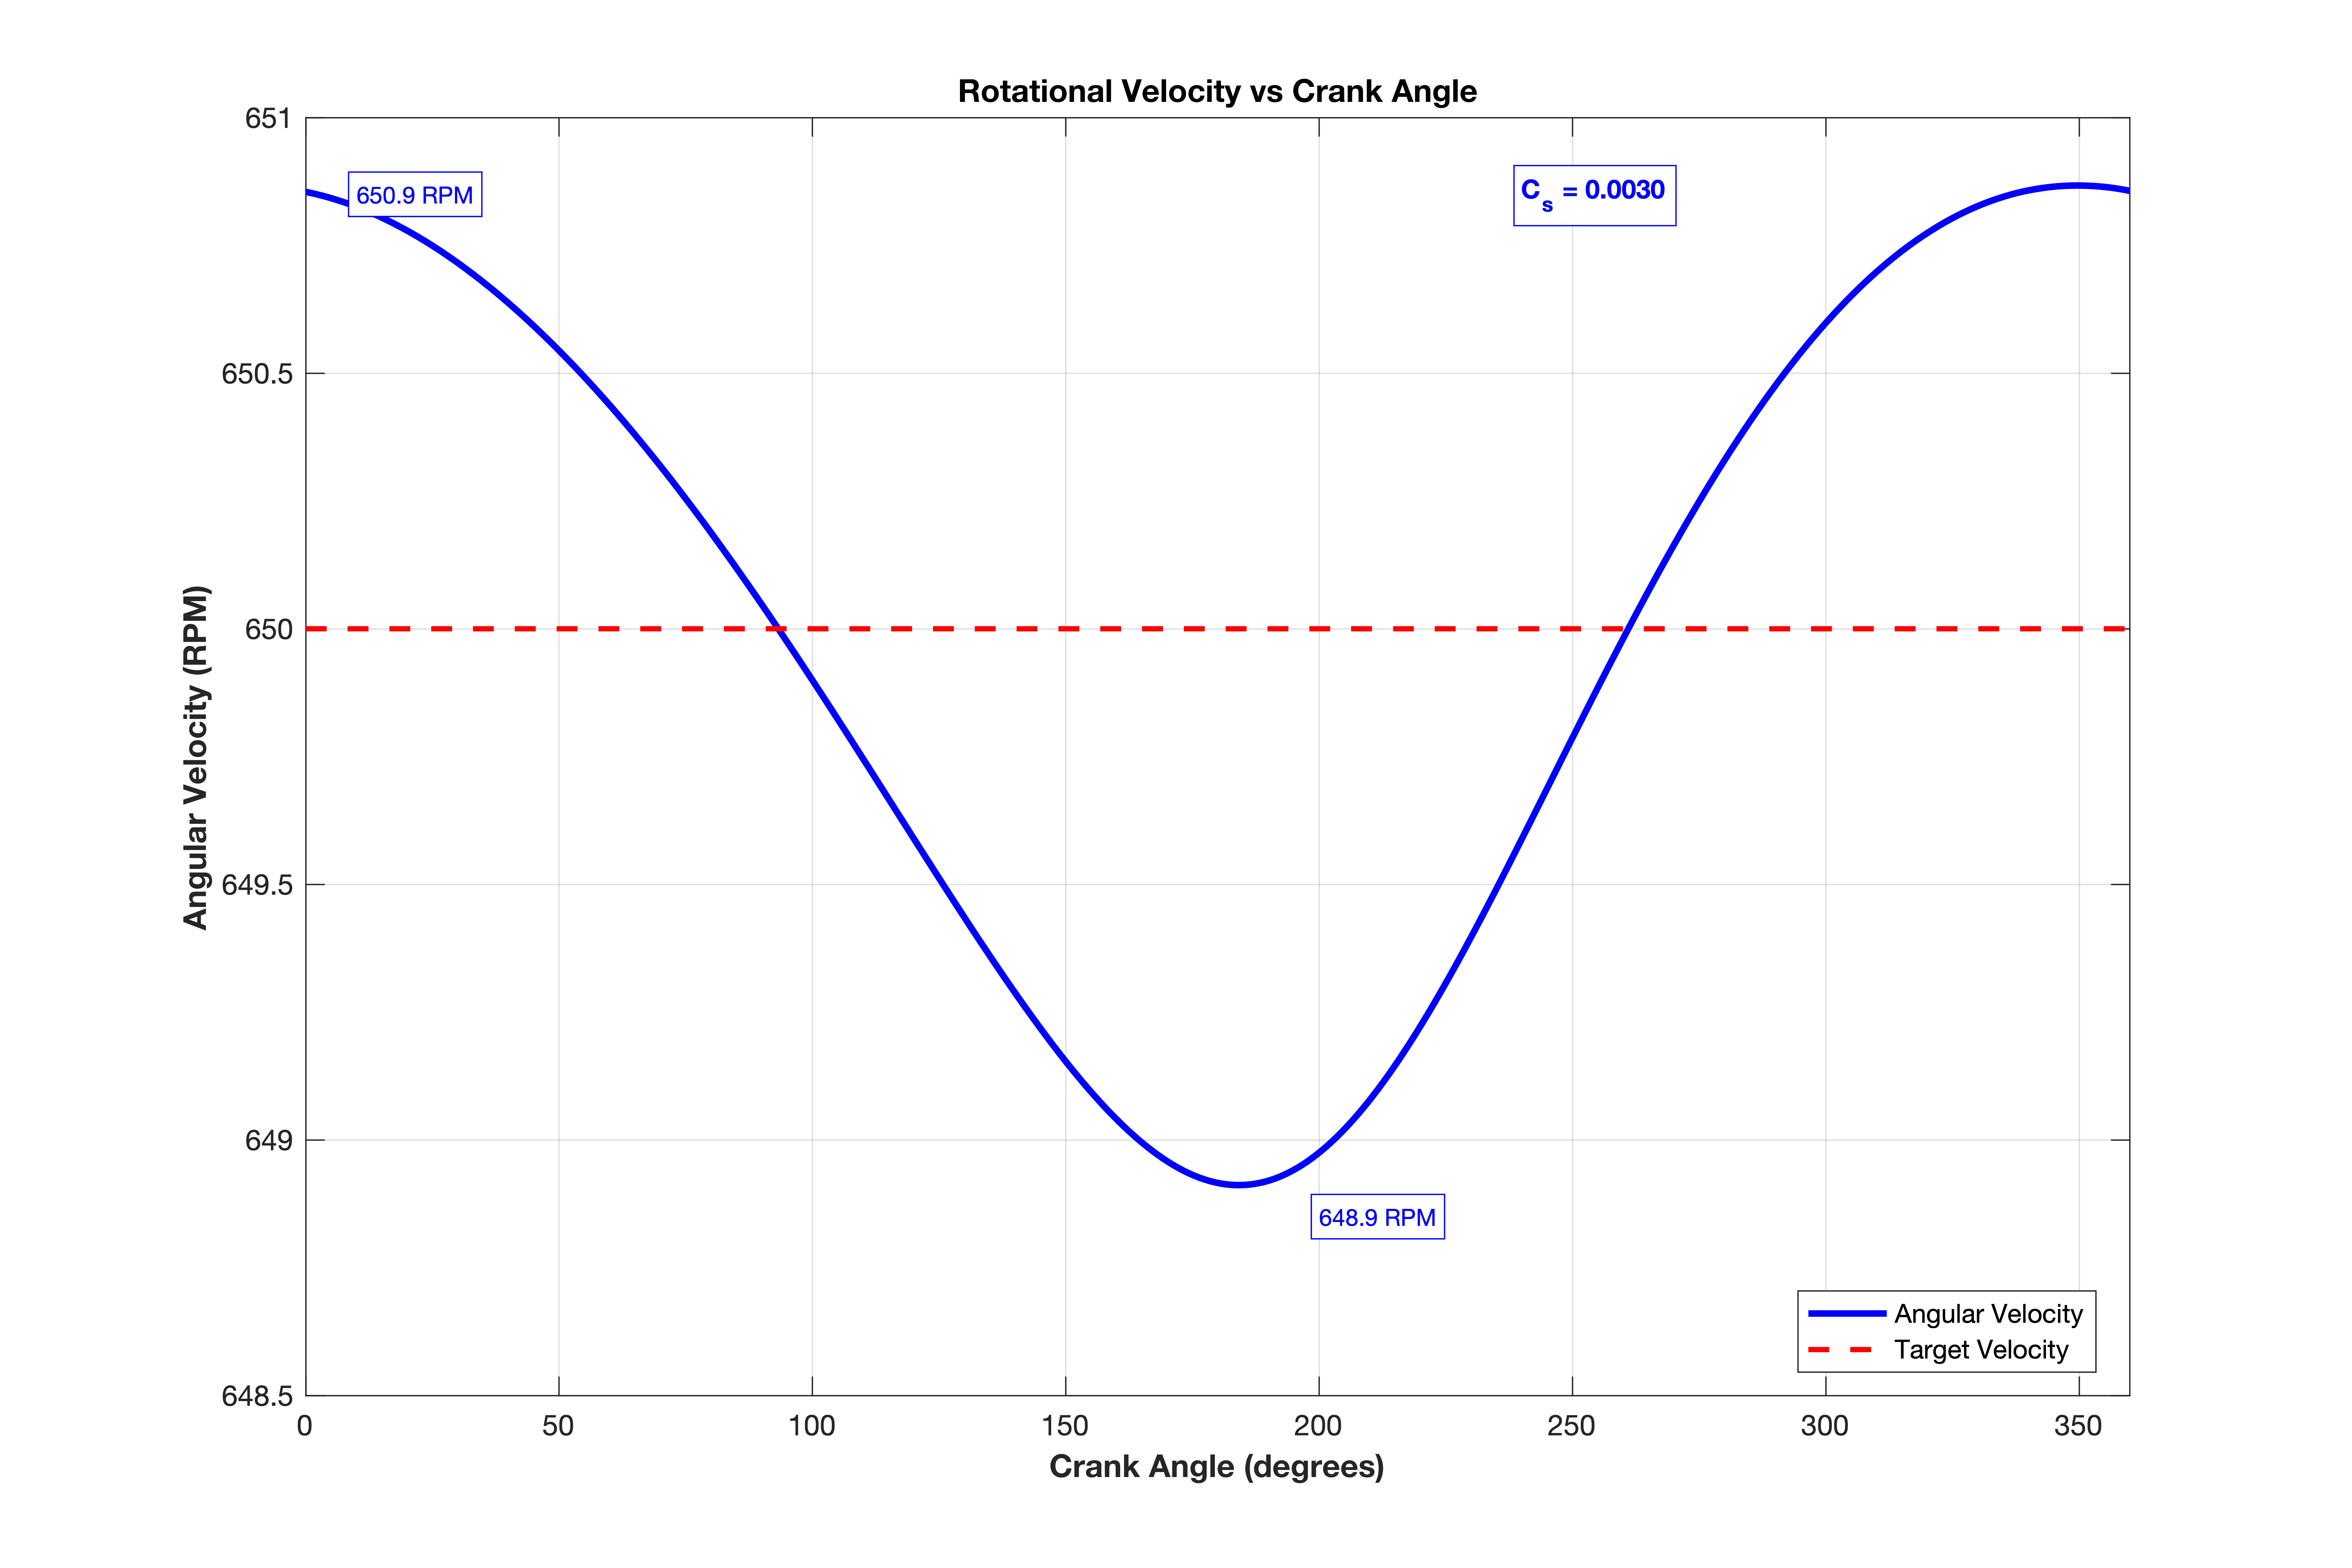
\includegraphics[width=0.8\linewidth]{../angular_velocity.png}
  \caption{Angular velocity vs. crank angle showing the speed regulation achieved by the flywheel.}
  \label{fig:angular_velocity}
\vspace{-6pt}\end{figure}

Operating at a target speed of 650 RPM, the engine maintains a velocity range of 648.9 to 650.9 RPM, achieving the target coefficient of fluctuation of 0.003. The maximum velocity occurs at 350.0°, while the minimum velocity occurs at 184.5°, demonstrating the flywheel's effectiveness in smoothing out torque variations.

The flywheel design requires a substantial moment of inertia of 4.48 kg·m², achieved through a flywheel with an outer diameter of 0.887 m, inner diameter of 0.787 m, and mass of 25.47 kg. These dimensions are consistent with typical flywheel designs for similar power levels and operating speeds.

\subsection{Phase Optimization Results}
The phase optimization analysis reveals the sensitivity of engine performance to phase shift, as shown in Figure~\ref{fig:energy_phase}.

\begin{figure}[H]
  \centering
  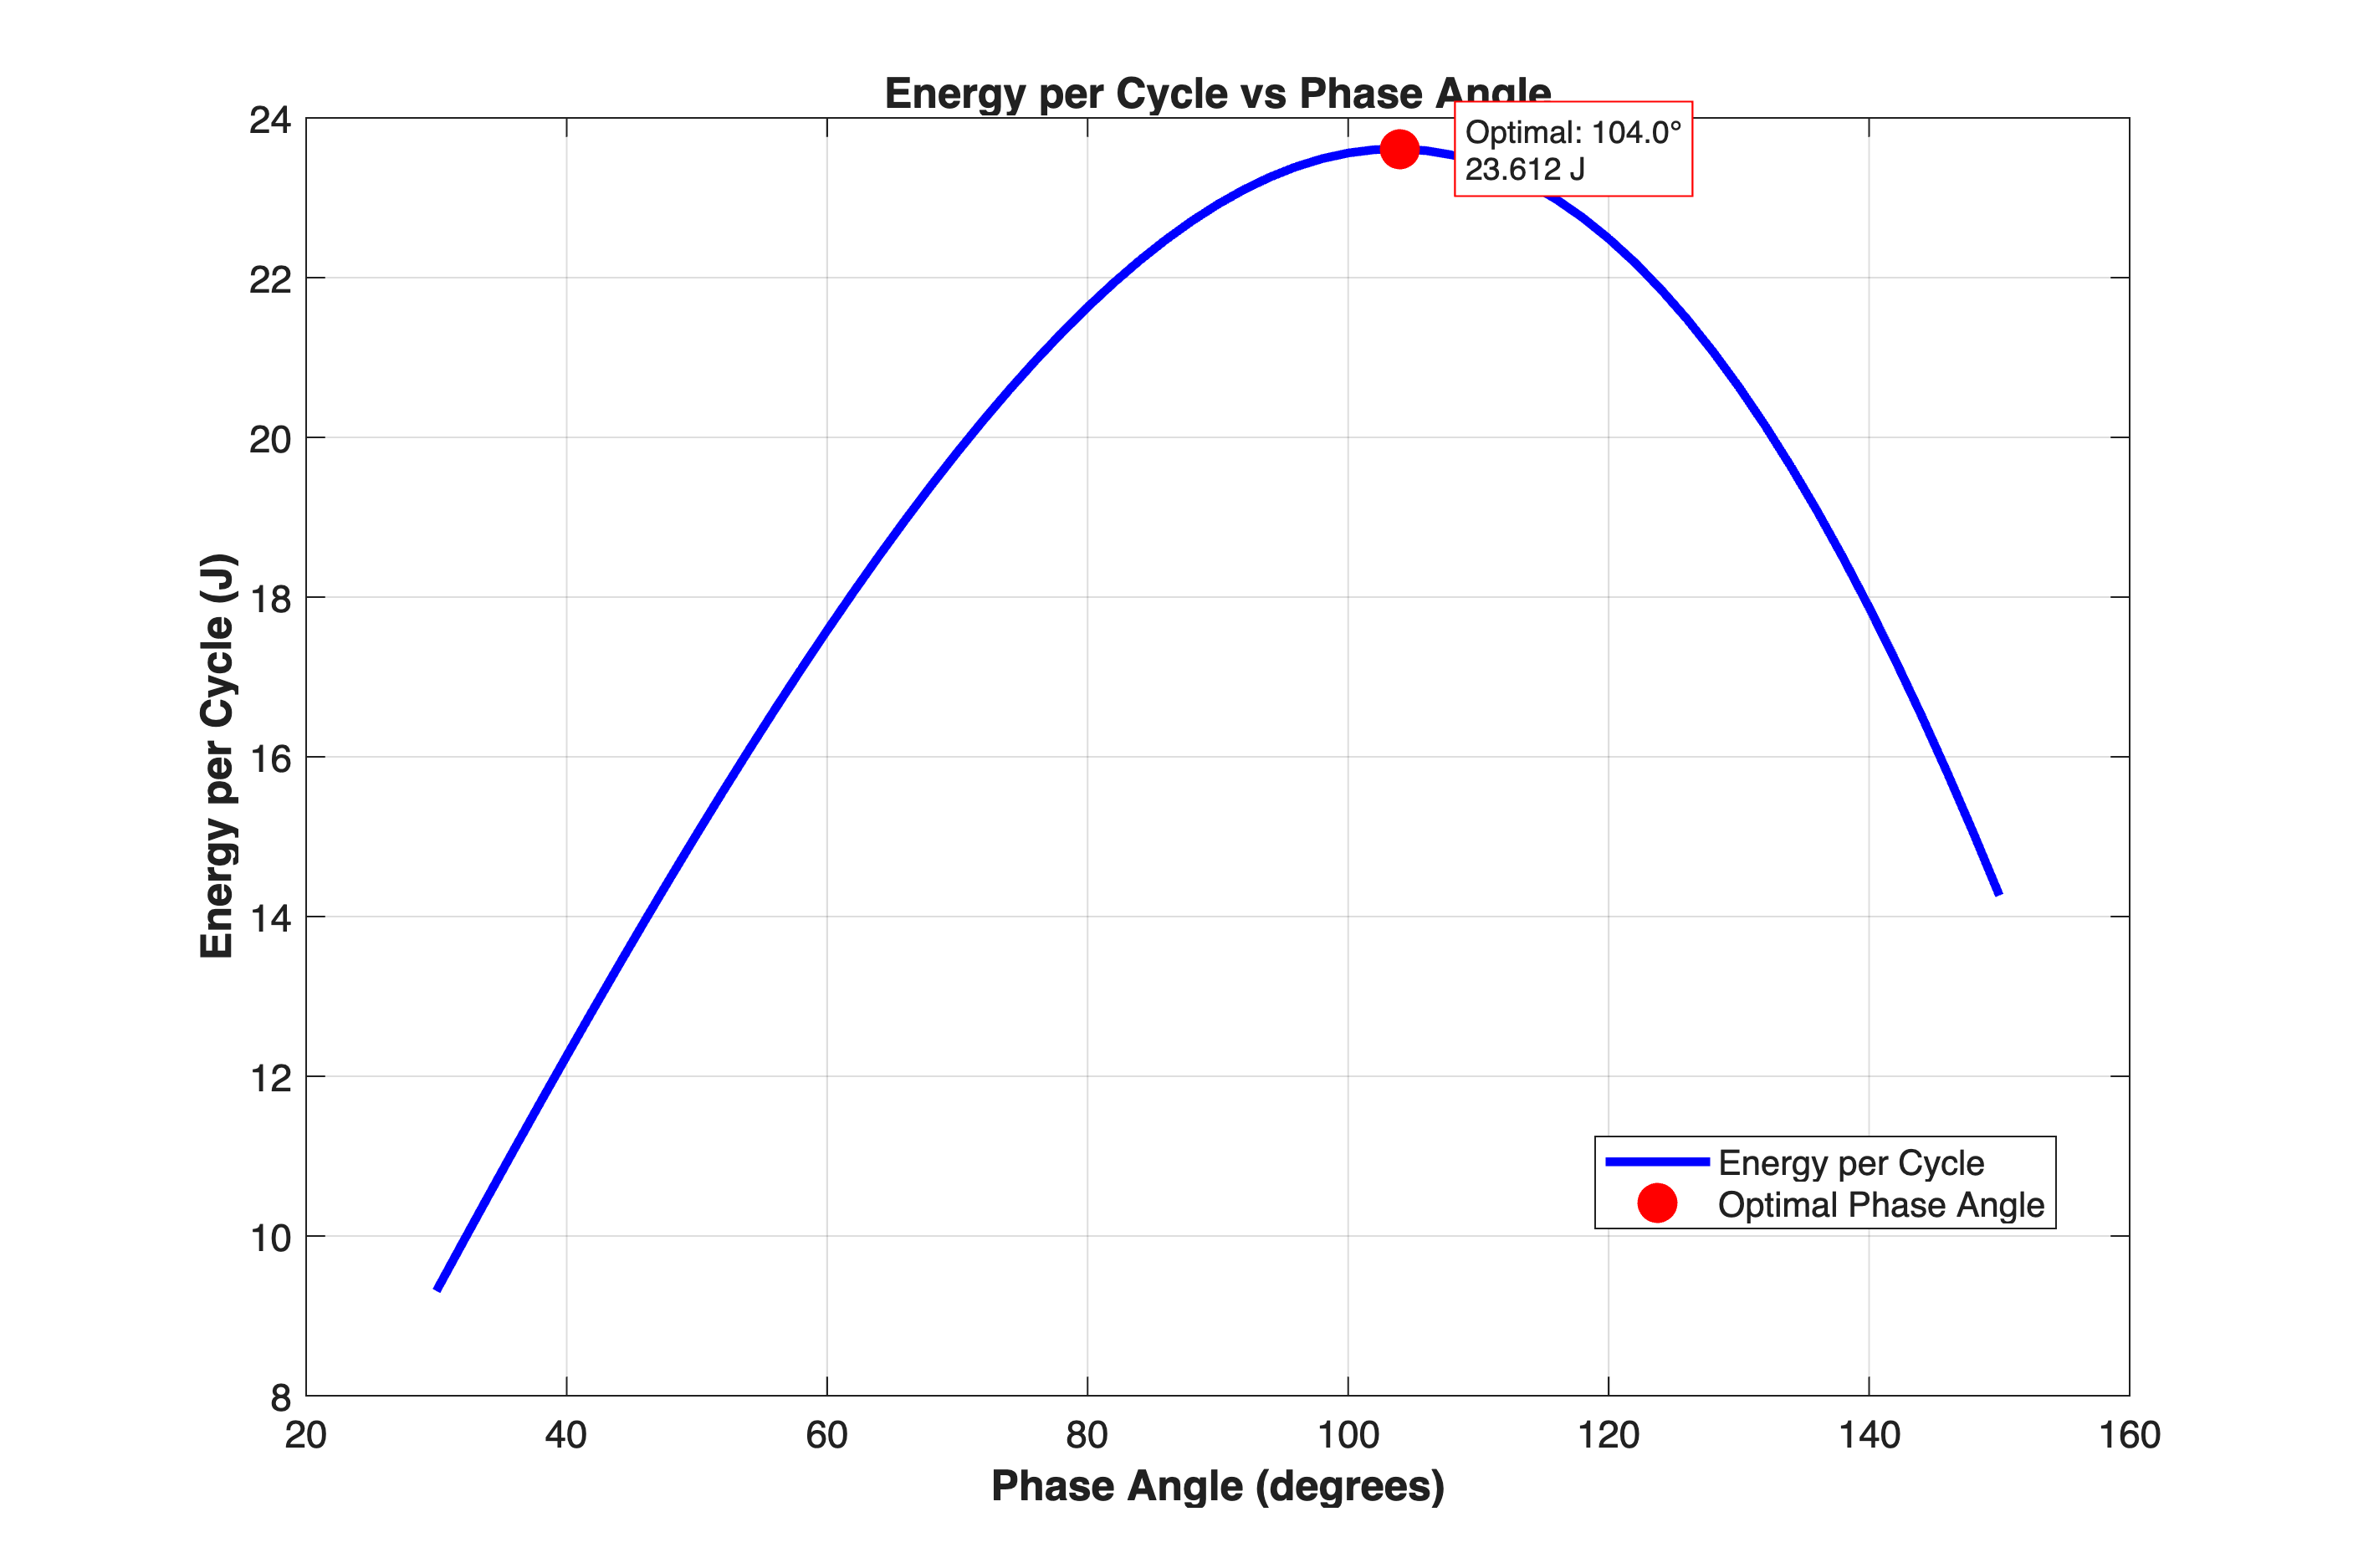
\includegraphics[width=0.8\linewidth]{../energy_vs_phase.png}
  \caption{Energy per cycle vs. phase angle showing the optimization results.}
  \label{fig:energy_phase}
\vspace{-6pt}\end{figure}

The optimization process reveals that the optimal phase angle of 103.6° provides maximum power output, which is 13.6° higher than the conventional 90° approximation. This deviation demonstrates the importance of systematic optimization rather than relying on simplified assumptions. The three-stage refinement strategy, achieving 0.01° resolution, ensures precise determination of the optimal operating point.

% (Condensed: key findings and requirement assessment are synthesized in the Conclusion to save space.)

\section{Conclusion}
This computational analysis successfully demonstrates the complete thermodynamic and dynamic behavior of a Beta-type Stirling engine through systematic modeling of piston kinematics, Schmidt analysis, and flywheel design optimization. The methodology establishes a comprehensive framework where all system variables—position, volume, pressure, torque, energy, and flywheel parameters—are expressed as functions of crank angle, enabling parametric studies and optimization.

\subsection{Thermodynamic Performance}
The pressure-volume analysis reveals significant performance characteristics for the given engine configuration. The ideal Stirling cycle produces 94.9 J of work per cycle, while the actual Schmidt analysis yields 23.0 J, resulting in a cycle efficiency of 24.2\%. This efficiency represents the ratio of actual work output to the theoretical maximum, indicating substantial losses due to non-ideal processes, dead volumes, and the simplified Schmidt assumptions. The positive mean torque of 3.648 N·m confirms the engine's ability to produce net work output over a complete cycle, validating the thermodynamic design.

\subsection{Phase Optimization Results}
Phase shift optimization reveals that the optimal phase angle of 103.6° provides maximum power output, which is 13.6° higher than the conventional 90° approximation. This deviation from the standard value demonstrates the importance of systematic optimization rather than relying on simplified assumptions. The optimization process employed a three-stage refinement strategy, ultimately achieving 0.01° resolution to ensure precise determination of the optimal operating point.

\subsection{Dynamic Behavior and Flywheel Design}
The angular velocity analysis shows excellent speed regulation with minimal fluctuation. Operating at a target speed of 650 RPM, the engine maintains a velocity range of 648.9 to 650.9 RPM, with maximum velocity occurring at 350.0° and minimum velocity at 184.5°. This 2.0 RPM variation corresponds to the target coefficient of fluctuation of 0.003, demonstrating effective flywheel performance.

The flywheel design requirements are substantial but reasonable for the system scale. A moment of inertia of 4.48 kg·m² is required, achieved through a flywheel with an outer diameter of 0.887 m, inner diameter of 0.787 m, and mass of 25.47 kg. These dimensions are consistent with typical flywheel designs for similar power levels and operating speeds.

\subsection{Engineering Implications}
The analysis demonstrates that while idealized assumptions (Schmidt analysis, isothermal processes) provide valuable insights into engine behavior, they significantly overpredict performance compared to real-world conditions. The 24.2\% efficiency indicates substantial room for improvement through enhanced heat transfer, reduced dead volumes, and more sophisticated thermodynamic modeling. The systematic approach developed here provides a foundation for parametric studies and design optimization of Beta-type Stirling engines, with the understanding that additional losses from heat transfer limitations, pressure drops, and mechanical friction would further reduce predicted performance in practical applications.
\end{document}
